% Current article. main.tex/named.pdf preserve the earlier cumulative report.
\documentclass[sigconf,dvipsnames,balance=false]{acmart}
\setcopyright{none}
\settopmatter{printacmref=false,printfolios=true}
\acmDOI{}
\acmISBN{}
\acmConference[Research draft]{Internal research draft in GECCO format}{20 October 2026}{}
\usepackage{algorithm}
\usepackage{algpseudocode}
\usepackage{xurl}
\usepackage{tikz}
\usetikzlibrary{arrows.meta,positioning}
\setlength{\emergencystretch}{2em}
\graphicspath{{../../figures/ManiGuard/latent-evolution/}}
\newcommand{\ind}{\mathbf{1}}
\newcommand{\safe}{S_{\mathrm{req}}}
\newcommand{\complete}{C_{\mathrm{req}}}
\begin{document}
\raggedbottom
\title{Evolving Native-Noise Controllers for Safe Completion with Frozen Manipulation Policies}
\subtitle{Completed frozen Jar pilot and separate continuation feasibility screen}
\author{Sachin Mohan}
\affiliation{\institution{University of the Witwatersrand}\city{Johannesburg}\country{South Africa}}
\email{2699183@students.wits.ac.za}
\renewcommand{\shortauthors}{Mohan}
\begin{abstract}
Can a compact controller recover safer task completion from a frozen generative
manipulation policy under a small interaction budget? Our 176-parameter adapter
adds a bounded four-dimensional offset to native noise using measured robot state,
executed input history and frozen image/text features. The VLA and native execution
contract remain fixed. A 320-call decoder audit on ManiGuard Jar and Clutter
passes all 32 same-noise identities and verifies action-prefix influence. Four
full development episodes establish integration and timing. A frozen 60-episode
study includes matched evolutionary and random-search adaptation and sixteen
protected independent checks. All sixty episodes are complete and independently
validated. All forty comparison-training trials remain requested-unfinished;
four nonviolating lid closures never extend to holding. In the four checking
cases per condition, every method has zero safe requested completions. Native and
EA each have three violations, versus two for fixed and random search. Their
raw goals occur only after violations and fail the requested sequence. Fixed and
random finalists have identical retained weights. This pilot establishes no
evolutionary safe-completion advantage. A separate 48-call decoder diagnostic finds
stronger-offset gripper influence with arm coupling. Four separately frozen
engineering trials then test native continuation after a closure-producing
controller on an exposed task and seed. All remain requested-unfinished: native
and closure-only are nonviolating; both handoffs violate and never satisfy native
holding. The privileged trigger fires, without a later ordered milestone. This
screen fails its expansion rule. A CPU model-assisted prototype also fails its
prediction/calibration audit and remains undeployed. Native-noise and evolutionary
VLA steering have precedents. Explained
safe completion per total interaction remains a contribution to establish; competent
learning comparisons, replication and transfer are still required.
\end{abstract}
\begin{CCSXML}
<ccs2012><concept><concept_id>10010147</concept_id>
<concept_desc>Computing methodologies</concept_desc>
<concept_significance>500</concept_significance></concept></ccs2012>
\end{CCSXML}
\ccsdesc[500]{Computing methodologies}
\keywords{evolutionary robotics, frozen policies, latent steering, safe manipulation}
\maketitle

\section{Introduction}
Completing a manipulation task and respecting its physical specification are
different outcomes. A robot may transport a jar with its lid open, or avoid every
violation while never finishing. ManiGuard makes these distinctions measurable
through task checks and passive runtime monitors~\cite{maniguard}. We investigate
whether a small controller can improve safe requested completion around its
family-specific frozen vision-language-action policies.

The adapter steers the generator's native noise before decoding an action chunk,
conditioning on current observations, the actual instruction and causal executed
action history. Evolution optimizes a small parameter matrix from complete
physical simulator outcomes. The VLA, feature encoder and native execution contract
remain fixed. This physical comparison deploys no learned safety filter, world
model or online action veto. Section~\ref{sec:model-followup} separately presents
implemented CPU preparation, its failed factual audit and the completed separate
continuation screen; those components do not alter the original comparison.

Earlier restraint/feedback pilots found limited trigger opportunities and no
safe-completion benefit~\cite{priorpilot}. Their different controllers and legacy
rendering profile are historical motivation, not controls for this experiment.

We separate four questions: does adaptation help native execution; does
conditioning help a fixed bias; does evolutionary retention and mutation help
relative to other adaptation methods; and do fitted weights transfer? Integration,
decoder influence, two adaptation generations and protected checking are complete.
The matched Jar comparison followed a protocol frozen before comparative feedback.
Its small sample gives a negative exploratory result, without optimizer-superiority
or cross-family-transfer evidence.

\section{Related work and contribution boundary}
DSRL learns in the latent-noise space of a frozen diffusion policy, including
generalist-policy adaptation~\cite{dsrl}. Flow Reversal Steering maps coarse
reference actions through a reversed flow and learns auxiliary noise policies;
it also studies repeated or averaged noise across chunk positions~\cite{frs}.
Principal Steering Subspaces constructs a low-dimensional basis from decoder
responses and controls its leading directions with SAC~\cite{pss}. Noise-space
adaptation, chunk repetition and low-dimensional steering are therefore not novel
by themselves. Our present basis is random and fixed, not response-informed.

Evolutionary VLA steering also has precedents. VLA-Pilot evolves action proposals
under an inferred steering objective during inference~\cite{vlapilot}. Online-ES
uses executed trajectory perturbations and feedback-weighted training to update
model parameters~\cite{onlinees}. Here the base VLA stays frozen while selection
updates a reusable conditional adapter using specification-labelled episode
outcomes. This defines an empirical question, not a priority claim. A conventional
EA or optimizer substitution alone is insufficient novelty.

The intended contribution is a reproducible, mechanistically explained improvement
in safe requested completion per total interaction. Evidence must distinguish
useful steering from a tuned constant, and evolutionary advantage from random
search and competent ordinary learning. One fitted adapter working with several
family checkpoints is the longer-term target. Reusing its interface with per-family
refitting is a weaker claim than transferring the same weights.

\section{Physical evaluation boundary}
At query time $\tau$, the frozen family policy decodes native Gaussian noise
$\epsilon_\tau\in\mathbb R^{16\times32}$ from two RGB views, robot input and
the prompt. Native output transforms produce physical joint-target/gripper
commands. The first eight are executed unless native termination occurs sooner.
The adapter changes noise rather than action horizon. Native is the same
family-fine-tuned policy with steering disabled. For Jar, both conditions use
the released LoRA checkpoint at step 7400; this pilot performs no new supervised
fine-tuning or zero-shot foundation-policy comparison.

Let $V$ be raw native \texttt{ltl\_violated}, without engagement gating. Requested
completion $\complete$ requires native success and the pinned family checklist.
For Jar, closure must be observed strictly before lifting, remain true at every
off-support observation and at the end, and lifting must occur. The final native
held/intersection goal must also hold. This stricter sequence check is reported
beside the unmodified benchmark verdict. Safe completion and training utility are
\begin{equation}
 \safe=\complete\land\neg V,\qquad U=\ind(\safe)-2\ind(V).
 \label{eq:utility}
\end{equation}
A violating completion scores $-2$; unfinished nonviolating execution scores zero.
This is a declared penalized objective. Reporting retains all four joint
completion/safety categories, raw violations and denominators. Contact/grasp
indicators contextualize unfinished episodes; fewer violations can reflect inactivity.

The monitor supplies evaluation labels and never changes commands. Monitor
predicates, object poses, task/family/checkpoint identifiers and goal state are
excluded from the adapter. Timeouts are valid outcomes, not infrastructure
failures, and do not alone identify their physical cause.

\begin{figure*}[t]
\centering
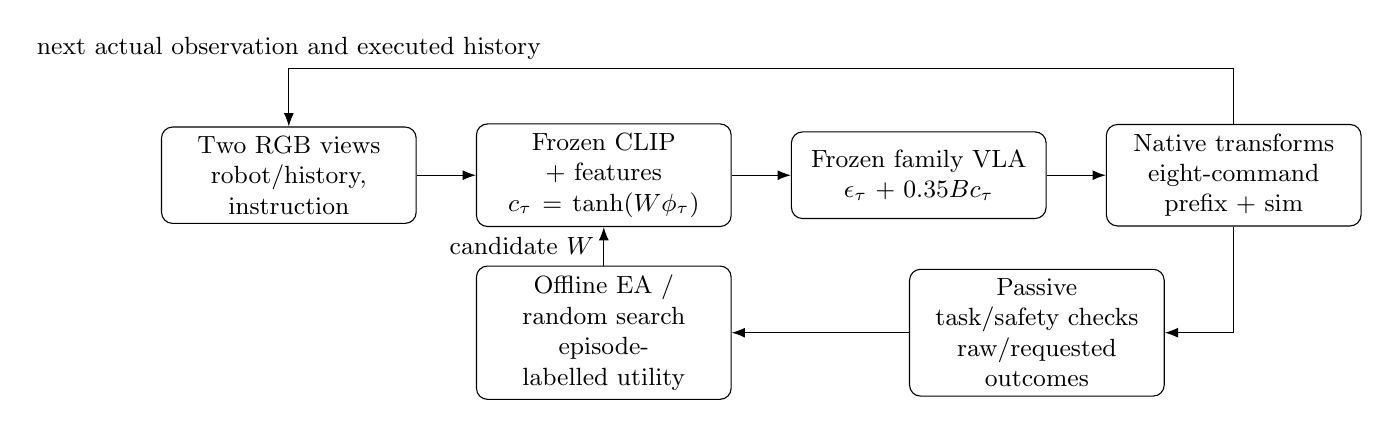
\begin{tikzpicture}[>=Latex,font=\small,
 box/.style={draw,rounded corners,align=center,minimum height=11mm,text width=30mm}]
 \node[box] (obs) at (0,0) {Two RGB views\\robot/history, instruction};
 \node[box] (adapt) at (4,0) {Frozen CLIP + features\\$c_\tau=\tanh(W\phi_\tau)$};
 \node[box] (policy) at (8,0) {Frozen family VLA\\$\epsilon_\tau+0.35Bc_\tau$};
 \node[box] (sim) at (12,0) {Native transforms\\eight-command prefix + sim};
 \node[box] (search) at (4,-2) {Offline EA / random search\\episode-labelled utility};
 \node[box] (monitor) at (9.5,-2) {Passive task/safety checks\\raw/requested outcomes};
 \draw[->] (obs) -- (adapt);
 \draw[->] (adapt) -- (policy);
 \draw[->] (policy) -- (sim);
 \draw[->] (sim.south) |- (monitor.east);
 \draw[->] (monitor) -- (search);
 \draw[->] (search) -- node[left]{candidate $W$} (adapt);
 \draw[->] (sim.north) -- ++(0,.7) -| node[pos=.5,above]{next actual observation and executed history} (obs.north);
\end{tikzpicture}
\caption{Implemented information boundary. Candidate weights are fixed within an
episode; the native Gaussian draw remains present. Outcome labels guide selection
of later candidates without vetoing execution. All conditions pay the same feature
extraction cost. The VLA also receives its unchanged native observation inputs.
No learned safety filter or world model is deployed.}
\Description{Observations feed a conditional noise controller and a frozen VLA.
Native execution feeds simulation. A passive monitor sends episode labels to the
offline search loop, which selects the next candidate controller.}
\label{fig:architecture}
\end{figure*}

\section{Native-noise controller}
\subsection{Causal features}
The feature vector $\phi_\tau\in[-1,1]^{44}$ comprises a bias, seven arm positions
divided by $\pi$, two measured finger positions divided by .04 m, seven previous
executed environment-input arm targets minus current arm positions divided by .2 rad, and three
end-effector displacements since the previous query divided by .05 m. Robot/history
coordinates are clipped. These targets precede downstream native-controller clipping;
they are neither achieved joint positions nor final motor commands. Initially the previous target equals measured joints and
displacement is zero.

The remaining 24 coordinates are eight each from overview RGB, wrist RGB and the
actual instruction. Frozen CLIP ViT-B/32~\cite{clip} produces 512-dimensional
embeddings. Each embedding is normalized to unit Euclidean norm. Fixed Gaussian-QR
projections, seeded 20261017, produce eight coordinates, multiplied by $\sqrt{512}$,
clipped to $[-5,5]$ and divided by five.
No feature fitting uses study outcomes. Images are encoded at every native query
and text once per episode, including in the native reference. The conditioning
path is implemented; its physical value is unestablished. A recorded-input audit
finds only two distinct training instructions and centered text-block rank one
across shared initialization. Text connectivity therefore does not establish
semantic generalization rather than case-specific offsets.

\subsection{Bounded steering with native stochasticity}
For genome $W\in[-1,1]^{4\times44}$, define $c_\tau=\tanh(W\phi_\tau)$ and
\begin{equation}
 z_{\tau,h}=\epsilon_{\tau,h}+.35Bc_\tau,
 \qquad h=1,\ldots,16.
 \label{eq:steering}
\end{equation}
The first seven rows of $B\in\mathbb R^{32\times4}$ are a reduced QR basis of
a Gaussian $7\times4$ matrix with PCG64 seed 20261019. Remaining rows are zero.
The offset repeats across the chunk and has Euclidean norm at most
$.35\sqrt4=.70$ per position in noise coordinates. This bounds sampling input,
not joint motion or violation probability. Gripper/padding noise are not directly
steered, but decoder coupling can affect their outputs. No persistence, learned
noise scale or activation gate is used.

For $W=0$, an explicit branch calls unchanged native \texttt{Policy.infer} without
an explicit-noise argument. Nonzero controllers preserve the native RNG split and
Gaussian draw before adding the offset. A zero noise tensor would define a different
policy. Receipts retain RNG transitions, noise/observation hashes, offsets, decoded
physical chunks and source hashes. The runtime logs steered proposals and final
environment inputs. It does not buy an additional unsteered chunk at every query;
same-noise comparisons are confined to the bounded decoder audit.

\subsection{Matched search}
Shared initialization evaluates identity, positive and negative constants, and a
uniform random conditional matrix on two cases. Constants set only
$W_{0,0}=\pm\operatorname{atanh}(.5)$, yielding $\pm.175$ along the first basis
direction. The random matrix uses seed 20261019. Both methods receive these same
eight episodes, counted once globally and attributed to both information budgets.
The better constant becomes the fixed reference, with ties selecting positive.
This tunes two declared constants, not an extensive fixed-policy baseline.

Each method evaluates two generations of four candidates on two common cases per
generation. Both freshly re-evaluate the previous cohort's best candidate. EA adds
three children from alternating top-two parents using iid Gaussian weight mutation
with standard deviation .25 and clipping to $[-1,1]$. Random search instead draws
three uniform matrices from the same domain, with the same retained-incumbent cost.
Ranking uses summed utility and stable identifiers for ties. Only the last complete
cohort supplies each finalist, preventing best-of-repeat promotion. Both method
RNGs use seed 20261020. Descendant execution interleaves methods at each candidate
slot, using EA/random at even slots and random/EA at odd slots. Lineage and
pending/completed evaluations are persisted.

\begin{algorithm}[t]
\caption{Frozen comparison after four development episodes}
\label{alg:comparison}
\begin{algorithmic}[1]
\Require Pinned policy, features, domain, cases, seeds and budget
\State Evaluate four shared controllers on two cases (8 episodes)
\State Select fixed reference from the two constants
\State Initialize EA and random search with the same scored data
\For{generation $g=1,2$}
 \State Propose both four-candidate cohorts, including incumbents
 \For{candidate slot $j=0,1,2,3$}
  \For{method in the frozen alternating slot order}
   \State Evaluate its candidate on two common cases
   \State Verify both physical receipts and record scores
  \EndFor
 \EndFor
 \State Rank each complete cohort for subsequent selection
 \State Preserve all attempts, ancestry, RNG and physical records
\EndFor
\State Seal native, fixed and the two final-cohort finalists
\State Check four conditions on four blocks (16 episodes)
\State Report outcomes, block differences, activity and costs
\end{algorithmic}
\end{algorithm}

\section{Prospectively frozen physical protocol}
\subsection{Scope and native execution}
Jar and Clutter provide development exposure; Cabinet and Dusty remain physically
untouched by this study. Jar/Stack/Lid/Clutter have programme-level history.
Jar is the primary pilot and Clutter the declared capacity fallback. The selected
protocol was frozen at 04:27:23 UTC on 20 October before comparative feedback,
using development timing and the authority criterion. It selects Jar. This pilot
does not train or test one shared cross-family adapter.

Execution uses native $640\times640$ DLAA rendering, two actual camera views,
the verified extended-finger Franka, assisted grasping, 20 Hz policy control,
60 Hz rendering and 120 Hz physics. Hard horizons are 2,000 controls for Jar and
1,100 for Clutter. Preprocessing, gripper binarization, native clipping and
termination are unchanged. Jar uses checkpoint step 7400, revision
\texttt{1d84eda07031}; Clutter uses step 7100, \texttt{f572e33bdb49}.
Full revisions and file hashes remain in study records.

Jar training tasks are 0019/0009, with base seeds $6101910+10g+i$, generation
$g=0,1,2$ and task index $i=0,1$. Checking tasks 0016/0012/0011/0003 use seeds
$6101940+i$. These blocks are reserved from this optimizer's feedback. Historical
validation allocation does not establish absence of earlier programme exposure;
we conservatively describe them as exposed tasks with independent checking.
The original main-study test partition remains excluded. Native per-scene
sampling-seed derivation is retained.

\subsection{Allocation and hardware balancing}
Table~\ref{tab:allocation} specifies the 60 planned valid full episodes. At most
four genuine infrastructure failures may be replaced, yielding a 64-full-attempt
ceiling. Every partial/invalid attempt and discarded candidate is charged. Valid
timeouts and adverse scores cannot be replaced. Separate engineering used six
starts: three failed during preparation and three reached 32 controls each.
The 96-control engineering allowance is exhausted. Physics before callback
attachment is unknown, not zero. The original 320-call decoder allowance is
exhausted. A separately authorized 48-call follow-up, reported below, changes
neither this physical allocation nor the controller used in the frozen comparison.

\begin{table}[t]
\caption{Frozen full-episode allocation. Shared initialization is acquired once.
The sixteen-episode independent check is protected from adaptation and tuning.}
\label{tab:allocation}
\begin{tabular}{@{}p{\dimexpr\columnwidth-65pt\relax}r@{}}
\toprule
Stage & Valid episodes \\
\midrule
Development, Jar + Clutter & 4 \\
Shared initialization: four controllers, two cases & 8 \\
EA: two generations, four candidates, two cases & 16 \\
Random search: same structure and domain & 16 \\
Independent check: four conditions, four blocks & 16 \\
\midrule
Planned total & 60 \\
Maximum starts with infrastructure replacements & 64 \\
\bottomrule
\end{tabular}
\end{table}

Two workers each colocate simulation and policy on one RTX 3090. Training case
$i$ uses worker $(i+g)\bmod2$ for both methods. Denoting native, fixed, EA and
random by $N,F,E,R$, checking orders are $(N,F,E,R)$, $(F,R,N,E)$,
$(E,N,R,F)$ and $(R,E,F,N)$. Adjacent pairs run concurrently; positions zero and two
use worker zero. Every condition therefore runs twice per GPU. One admission
ledger enforces the global attempt ceiling. Process identities and terminal
receipts permit reattachment without duplicate physical launches.

Capacity protects 56 post-development episodes plus four replacement slots as 30
two-worker waves. Its per-wave bound is the maximum of 180 s, 1.25 times the
slowest complete development process, and a startup-plus-native-horizon throughput
estimate with the same margin. Including 900 s for lifecycle/preservation, Jar
requires 15.008 h. The original window was insufficient; the user subsequently
authorized the full comparison on this instance. The fixed cutoff is 19:30 UTC
and independent local stop 20:00 UTC on 20 October. Horizons/rendering were not
reduced to fit.

\subsection{Analysis and uncertainty}
The final comparison retains all four requested completion and safety categories
and raw benchmark completion per condition, with paired differences by checking
block. Initial robot/image hashes are checked: common seeds do not prove identical
camera observations. Contact/grasp indicators contextualize noncompletion.
Cost curves use common cumulative physical control counts and retain all adaptation,
failures and discarded candidates. Model calls, encoder work, elapsed time and
allocated GPU-hours are separate counters. Shared episodes count once physically
and once within each method's information budget.

Setup, decoder calls, idle allocation and preservation are charged. GPU-hour and
running-cost estimates are upper bounds over elapsed wall time from the original
provider start, counting both GPUs. The own-instance API does not expose verified
billed runtime; a container restart is not credited as unbilled time. Four checking episodes
per condition and one optimizer seed provide descriptive effect sizes, not a
superiority or safety guarantee. Zero violations in $n$ independent episodes
implies an approximate 95\% upper rate bound of $3/n$, not zero; four episodes
are particularly weak evidence.

\section{Completed physical and decoder evidence}
The complete original60 export is dated 20 October, after all forty training,
four development and sixteen protected checking trials completed. Its full design
verification and private-archive physical replay pass. The separately frozen
four-start engineering screen is also complete and is reported separately below.
\subsection{Identity and decoder influence}
Eight saved observations per family, from two development tasks, each use two native
noise draws. Each draw receives two same-noise baselines and positive/negative
offsets along four directions: ten calls and 320 total. All sixteen identity pairs
per family pass the declared $10^{-5}$ absolute/relative tolerance. Full remote
recovery also reproduces noise hashes and RNG transitions without new model calls.

\begin{figure}[t]
\centering
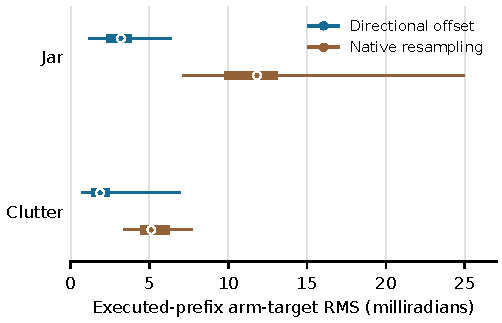
\includegraphics[width=\linewidth]{decoder-authority.pdf}
\caption{Arm-target RMS differences over the executed eight-command prefix.
Thick intervals show quartiles, thin intervals the range and circles the median.
There are 128 directional comparisons and eight native-resampling comparisons per
family, clustered within eight saved observations. These are decoder responses,
not independent physical trials or safety measurements.}
\Description{Jar perturbation median is .00319 rad versus .01183 for native
resampling; Clutter medians are .00187 and .00512 rad, respectively.}
\label{fig:authority}
\end{figure}

Perturbed-prefix arm RMS ranges from .001131 to .006422 rad for Jar, median
.003193, and .000666 to .006975 rad for Clutter, median .001868
(Figure~\ref{fig:authority}). Native-resampling medians are .011827/.005118 rad.
All four directions per family pass the frozen criterion: observation-level mean
RMS at least .001 rad on at least half the observations, with two passing
directions required. The smallest individual Clutter response need not exceed
this observation-level threshold. No executed-prefix gripper flips occur among
128 directional probes per family. Coupling elsewhere is not excluded.

A 32-control Clutter integration check uses an untrained dense conditional matrix,
exercising all 176 weights including 96 semantic weights. Removing semantic
features offline changes its code by RMS .3781 on factual observations. This
verifies a software path, not semantic competence or a physical counterfactual.

\subsection{Full development outcomes}
Table~\ref{tab:development} preserves four full episodes on different tasks/seeds.
Their native/bias differences do not estimate an adaptation effect. Jar native
reaches the raw benchmark goal but fails the closed-lid sequence: requested unsafe
unfinished, versus raw unsafe completion. Jar bias and Clutter native reach their
full horizons, both valid outcomes rather than replaceable failures.

\begin{table}[t]
\caption{Full development episodes. $C$ is requested completion, $V$ raw
violation, $A$ controls and $Q$ policy calls. Each row uses a different task/seed.}
\label{tab:development}
\begin{tabular}{llrrrrr}
\toprule
Family/controller & Task & $A$ & $Q$ & $C$ & $V$ & $U$ \\
\midrule
Jar native & 0013 & 666 & 84 & 0 & 1 & $-2$ \\
Jar positive bias & 0017 & 2000 & 250 & 0 & 0 & 0 \\
Clutter native & 0039 & 1100 & 138 & 0 & 1 & $-2$ \\
Clutter negative bias & 0010 & 532 & 67 & 1 & 0 & 1 \\
\bottomrule
\end{tabular}
\end{table}

Development closeout contains ten starts, 4,394 controls, 4,464 environment steps
and 26,987 known physics ticks. There are 551 physical-policy calls and 320 decoder
calls. Encoding records 1,102 images, seven text calls, 23.519 s extraction and
38.443 s loading; physical-policy request wall time is 293.776 s. These totals
precede the comparison and are not final study costs. Callback-unobserved
initialization physics remains unknown.

Clutter native has a 574.6 s cold startup versus its partner's 99.9 s. Logs identify
a locked shared Kit cache and shader compilation. The episode then completes
normally and retains its cost in capacity selection. This technical delay is
distinct from its valid adverse physical outcome.

\subsection{Completed shared initialization}
All eight shared initialization episodes reach the full 2,000-control horizon
without requested or raw benchmark completion (Table~\ref{tab:initial}). Each
controller receives the same two nominal task/seed cases, costing 4,000 controls
and 500 policy calls. Shared acquisition therefore costs 16,000 controls and 2,000
policy calls globally, attributed once within each optimizer's information budget.

\begin{table}[t]
\caption{Shared training initialization, two episodes per controller. SC/UC are
safe/unsafe requested completion; SU/UU are safe/unsafe unfinished episodes.
$V$ counts violations and $G$ episodes with a recorded grasp. Random here is
the shared untrained conditional initializer, not a selected random-search finalist.}
\label{tab:initial}
\begin{tabular}{lrrrrrr}
\toprule
Controller & SC & UC & SU & UU & $V$ & $G$ \\
\midrule
Native & 0 & 0 & 1 & 1 & 1 & 1 \\
Positive constant & 0 & 0 & 1 & 1 & 1 & 0 \\
Negative constant & 0 & 0 & 2 & 0 & 0 & 0 \\
Random conditional & 0 & 0 & 0 & 2 & 2 & 0 \\
\bottomrule
\end{tabular}
\end{table}

The negative constant's utility sum zero leads native and positive at $-2$ and the
random initializer at $-4$. It never grasps and contacts the target in only one
of its two episodes. This lead concerns nonviolating unfinished execution, not
improved safe completion. The frozen rule selects it as the fixed reference and
initial incumbent of both searches. Native task 0019 goes off support while open
at action 537; closure first becomes true at 638. Positive task 0009 instead loses
uprightness at 1116 while still supported, with no recorded grasp. These are
factual failure descriptions, not counterfactual explanations of a steering effect.

The initial robot input matches native in all six comparisons of a different
controller on the same case. Both RGB views differ in every pair. Stored native-noise hashes and RNG
transitions agree at all 1,500 paired query indices across those six streams.
The common random stream is realized while observations remain different. These
are correlated consistency checks over two cases, not independent outcome trials.

\subsection{Exploratory gripper-coordinate diagnostic}
Four generation-one incumbent rechecks subsequently evaluate the same negative
constant on the new training seed panel. Each method scores $[0,-2]$: no requested
or raw completion and one violation per pair. At this diagnostic cutoff, all
twelve comparison episodes are unfinished, six violate, and only one ever grasps.
Eight never command gripper closure; the other four each show actual finger
closure. None of their arm proposals changes at the outer environment bounds.
These observations did not identify a unique failure cause. Offspring evaluation
was still pending at that earlier diagnostic boundary; its completed first
generation is reported below.

The frozen basis excludes direct support on the gripper-noise coordinate. During
a diagnostic pause, a separately frozen 48-call follow-up tests coordinate seven
(zero-based) on eight saved middle/last development frames, four per family from
two episodes. Each input receives a native draw, an explicit same-noise repeat
and offsets $\pm0.5$ and $\pm2.0$ on that coordinate at all sixteen chunk positions.
No simulator or encoder runs. This raises total decoder requests to 368 while
retaining the original audit and physical cohort unchanged. All eight additional
same-noise identities pass at the original $10^{-5}$ tolerance.

\begin{table}[t]
\caption{Supplemental gripper-noise influence. Entries count saved observations
with at least one binarized gripper-command flip in the first eight decoded
actions under either sign. The last column is the largest arm-target difference
across those positions and the $\pm2.0$ probes. These are correlated decoder inputs,
not physical outcome trials.}
\label{tab:gripper}
\begin{tabular}{lrrr}
\toprule
Family & Magnitude 0.5 & Magnitude 2.0 & Max arm (rad) \\
\midrule
Jar & 0/4 & 3/4 & .05875 \\
Clutter & 0/4 & 4/4 & .01773 \\
\bottomrule
\end{tabular}
\end{table}

The stronger offset changes gripper commands in both families
(Table~\ref{tab:gripper}), with accompanying arm changes. Its positive sign opens
the gripper in all four Clutter frames, including two factual held-target frames;
its negative sign closes it in the two unfinished Jar-bias frames. Conditional
timing and physical benefit remain untested. Three inputs already lie on violating
factual trajectories, and no Jar input demonstrates a successful closure
transition. A flip there cannot establish prospective violation prevention. This
is influence in a candidate new representation, with no repair applied to the
frozen physical controller.

An independent offline sensitivity analysis uses 3,334 factual Jar query rows and
205 Clutter rows from completed development/training episodes. The three persisted
EA mutations change their parent codes by RMS .5410/.5825/.4130 on the Jar pool;
only .990\%/1.110\%/.127\% of their code components have magnitude at least .95.
Inactive mutation or general tanh saturation is therefore unsupported as the
current explanation. These are noise-space sensitivities on correlated factual
inputs, with longer trajectories weighted more. They do not measure decoded
actions, semantic competence or physical counterfactual benefit.

\subsection{Completed training and ordered progress}
All sixteen first-generation episodes reach 2,000 controls and 250 policy calls.
Neither method records requested or raw completion or a grasp. Each has four
violating and four nonviolating unfinished episodes, seven contact episodes and
population utility sum $-8$ (Table~\ref{tab:training-generations}).

\begin{table}[t]
\caption{Eight paid training episodes per row, including incumbent rechecks.
Requested safe/unsafe completions are zero throughout. SU/UU are safe/unsafe
unfinished; every UU has a raw violation. $G$ counts native target holding,
$L$ nonviolating supported closure and $B$ raw benchmark completion.
The sole raw goal is unsafe and requested-unfinished.}
\label{tab:training-generations}
\begin{tabular}{llrrrrr}
\toprule
Gen. & Method & SU & UU & $G$ & $L$ & $B$ \\
\midrule
1 & EA & 4 & 4 & 0 & 1 & 0 \\
1 & Random & 4 & 4 & 0 & 1 & 0 \\
2 & EA & 6 & 2 & 0 & 1 & 0 \\
2 & Random & 6 & 2 & 1 & 1 & 1 \\
\bottomrule
\end{tabular}
\end{table}

The last EA child wins the cohort with utility zero, versus random search's
best $-2$. Its first case closes the lid on support at observation 1,187 but never
grasps; its second never contacts the jar. This is a training-utility lead through
nonviolating unfinished execution, not a safe-completion benefit. Random draw 2
closes safely at observation 482 and remains supported and closed through 2,000,
but likewise never grasps. It ties all random candidates under the frozen utility;
stable identifier ordering correctly retains the incumbent rather than rewarding
this undeclared milestone.

Across the eight shared initial and sixteen first-generation episodes, none
completes, twelve violate and only the initial native episode ever grasps. The
twelve safe unfinished episodes comprise ten without an ordered milestone and
two with supported lid closure only. Nine comparison episodes issue closing
gripper commands, but none after safe supported closure. These factual complementary
partial behaviours motivate a separately declared continuation test; they do not
establish composability or uniquely diagnose failure. Milestone rewards, tie-rule
changes and transfer of a random-search controller into EA would change the method
and are excluded from this comparison.

On the second frozen seed panel, both methods have two violations, six safe
unfinished episodes and population utility $-4$. EA contacts the jar in six cases
and random search in five. Both incumbents score $[0,0]$ without closure or holding;
one case in each never contacts the jar. The earlier EA utility lead does not
persist on this common panel. New EA/random children close safely at observations
1,157/1,115, again without holding. All four nonviolating closure examples concern
task 0019 across two nominal seed panels, using different matrices.

Random's last child on task 0009 first loses uprightness at 788 while supported,
before holding at 833 and lift at 837. Closure never occurs. Raw goal at 1021 and native
termination at 1030 follow that violation, so utility remains $-2$. This demonstrates
holding in an unsafe context, not safe composition with another case's closure.
Across all forty comparison-training trials, sixteen violate and twenty-four
are safe unfinished; none completes the requested sequence. The sealed EA
finalist retains its first-generation winner; random retains the negative
constant, identical to the fixed reference. Selection uses only the frozen
utility and identifier tie rule. All sixteen independent checks are now complete.

\subsection{Completed independent checking}
Table~\ref{tab:checking} reports the sealed finalists on four nominally paired
Jar task/seed blocks, tasks 0016, 0012, 0011 and 0003. These cases were protected
from this optimizer's training, but retain the programme's earlier exposure;
they are not the untouched main-study test set. Every requested completion is
false. Native's raw goal on task 0003 and EA's on task 0012 follow violations
and remain requested-unfinished.

\begin{table}[t]
\caption{Independent checking, four episodes per condition. SC/UC and SU/UU
retain requested completion/safety categories. $V$ counts violating episodes,
$B$ raw benchmark goals and $G$ episodes satisfying the native holding predicate,
without an independent body-link grasp witness.}
\label{tab:checking}
\begin{tabular}{lrrrrrrrr}
\toprule
Condition & SC & UC & SU & UU & $V$ & $B$ & $G$ & Mean $U$ \\
\midrule
Native & 0 & 0 & 1 & 3 & 3 & 1 & 1 & $-1.5$ \\
Fixed & 0 & 0 & 2 & 2 & 2 & 0 & 0 & $-1.0$ \\
EA & 0 & 0 & 1 & 3 & 3 & 1 & 1 & $-1.5$ \\
Random & 0 & 0 & 2 & 2 & 2 & 0 & 0 & $-1.0$ \\
\bottomrule
\end{tabular}
\end{table}

The six candidate-minus-reference mean utility differences are fixed/native
$+0.5$, EA/native $0$, random/native $+0.5$, EA/fixed $-0.5$, random/fixed $0$
and random/EA $+0.5$. Every safe-completion difference is zero. Nonzero utility
differences arise solely from the violation difference on task 0011. Native and
fixed contact the target in all four cases, EA and random in three. This does
not establish why the differing failures occur. Fixed and random are the same
genotype: random retains the initial fixed controller through both generations;
EA retains its first-generation child unchanged in generation two. These are
retained lineages, not independent discoveries. Four blocks and one optimizer
run establish no evolutionary benefit or safety-rate guarantee.

The eight-value initial robot inputs match within every block. All non-native
initial camera pairs differ at some pixels, but each camera's mean absolute
channel difference, with RGB normalized to $[0,1]$, is below $1/255$.
Ten of twelve case comparisons have both
camera 99th-percentile differences at most $1/255$. Saved-view inspection finds
no visible object or camera relocation. Full simulator-state equality, the
cause of pixel variation and its policy sensitivity remain unestablished.

All sixty valid episodes plus six engineering starts, including failures,
cost 112,131 policy controls, 14,019 physical-policy requests, 112,761 returned
environment steps and 678,393 known physics ticks. The separate 368 decoder
requests bring neural policy returns to 14,387, with no failed or incomplete
server return. Feature extraction records 28,038 images and 63 text encodings.
The manual short engineering start is counted once; pre-callback initialization
physics remains unknown. At the original accounting boundary, elapsed rental
time gives 41.091 allocated GPU-hours over both GPUs and a \$12.586 upper-bound
estimate at the observed rate, including setup, idle time and preservation.
This is not verified billing or final rental closure. Later analysis and the
separate follow-up retain their own allocation accounting. CPU work is separate.

\section{Continuation screen and model-assisted preparation}
\label{sec:model-followup}
\textbf{Status: four physical engineering trials complete; CPU model fails qualification.}
These separate investigations change no original candidate, objective or checking
result. The physical screen tests a composition hypothesis on one exposed case;
the learned model and action-changing filter remain undeployed.

\subsection{Prospectively frozen continuation method}
Before original independent checking, we froze random-search draw 2 from generation
one, task 0019/base and exposed seed 6101920. Its earlier factual closure at 482
motivates this engineering case. All four references share that selected matrix
and development information: native only, closure only, fixed-clock handoff and
privileged supported-closure handoff. This tests feasibility, without a fresh-seed
generalization or EA claim. The clock adds elapsed-query information beyond the
original 44 actor coordinates; privileged gating additionally uses monitor labels.

The privileged trigger requires three consecutive post-control observations with
closed lid, support and no preceding violation. Observation zero is excluded.
Loss of qualification before the next eight-control query cancels the trigger.
Switch there and latch native execution, preserving the policy Gaussian stream,
episode identity and seed. The fixed clock is 488 from the exposed example.
Native and closure-only references make no switch. Every condition retains the
same encoder schedule, native termination and full 2,000-control horizon.

The four-total-start cap includes partial failures, with no automatic replacement
or extra decoder probe. Each start has independent startup/full-wall guardians,
durable admission and exclusive policy-service ownership. Original60 completion,
full restoration, unchanged source and fresh machine/rate/armed-clock/capacity
checks passed before dispatch. The compound reader verifies actual components,
RNG continuity, executed commands, exact native monitor entries and captured
server returns. Software preparation used 74 synthetic sampler calls, separately
from the 368 neural decoder-only calls.

A later stage requires a positive closure prefix and actual native continuation,
no whole-episode violation, and a new ordered holding/lift/transport milestone
strictly after switching or first safe requested completion after switching.
At-switch observations belong to the prefix. Holding uses the native predicate
without an independent body-link grasp witness. This criterion authorizes no
automatic extra starts; none of the actual references meets it.

\subsection{Completed physical screen}
All four starts reach 2,000 controls and pass full verification, with no invalid
start (Table~\ref{tab:screen}). No requested/raw goal or native holding occurs.
Native never contacts the target. Closure-only contacts it and first closes at
observation 596, remaining nonviolating with 1,405 closed observations, without
holding. This repeats partial closure on the selected exposed seed.

\begin{table*}[t]
\caption{Separate engineering screen: one full trial per mode, on the same exposed
task/seed. SC/UC and SU/UU are requested completion/safety categories; $V$ is the
whole-episode violation. Stage is the highest ordered milestone before any
violation; stage 1 is supported closure. $A_{\rm post}$ counts actual native
controls after a switch; native-only has no switch and executes 2,000 native
controls. $t_V$ is the first violating observation; $N_{\rm close}$ counts executed
closing inputs. These four cases establish no rate, causal effect or transfer.}
\label{tab:screen}
\begin{tabular}{lrrrrrrrrrr}
\toprule
Mode & SC & UC & SU & UU & $V$ & Stage & Switch & $A_{\rm post}$ & $t_V$ & $N_{\rm close}$ \\
\midrule
Native & 0 & 0 & 1 & 0 & 0 & 0 & n/a & 0 & n/a & 0 \\
Closure-only & 0 & 0 & 1 & 0 & 0 & 1 & n/a & 0 & n/a & 0 \\
Clock handoff & 0 & 0 & 0 & 1 & 1 & 0 & 488 & 1512 & 475 & 40 \\
Privileged handoff & 0 & 0 & 0 & 1 & 1 & 1 & 448 & 1552 & 471 & 142 \\
\bottomrule
\end{tabular}
\end{table*}

Clock execution loses uprightness while still supported and open at observation
475, before switching at 488. Its later first closure at 531 follows that
violation and earns no safe ordered credit. Privileged execution closes at 445,
debounces at 447 and switches at 448. It loses uprightness at observation 471,
23 native controls later, while still closed and supported. These timings do
not identify an action-specific cause; clock's first violation cannot be
attributed to its later handoff. Neither trial adds ordered holding, lift or
transport. There is no late native-goal confirmation to satisfy the alternative
completion-after-switch criterion. The screen is not expanded.

\begin{figure*}[t]
\centering
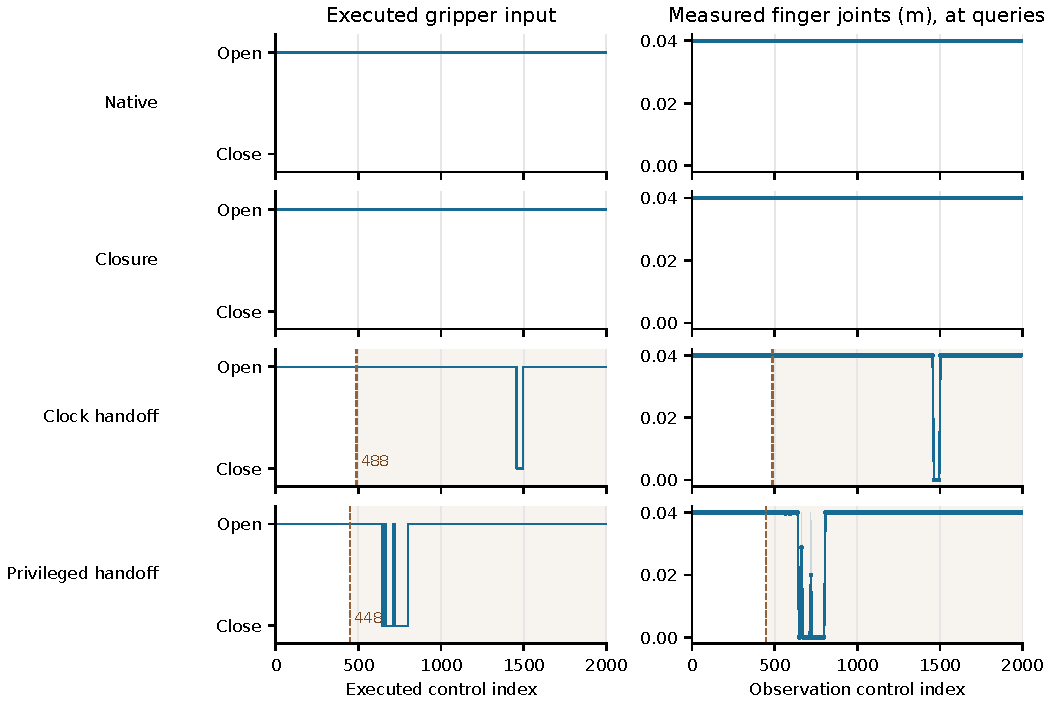
\includegraphics[width=\textwidth]{../../figures/ManiGuard/continuation-screen-20261020/gripper-trajectories.pdf}
\caption{Actual gripper inputs and measured query-time finger joints in the four
completed engineering trials. Dashed lines mark actual switches; tan regions
show native continuation. At-switch positions precede the first native action.
Points are two-joint means and blue bands span the two joints, without implying
uncertainty, fingertip aperture or a body-link grasp. A closing input does not
prove holding. Every plotted trace is bound to the completed physical audit.}
\Description{Native and closure-only command opening throughout. Both handoffs
later command closing and reach near-zero finger joints, without native holding.}
\label{fig:screen-gripper}
\end{figure*}

Native and closure-only command opening throughout, with finger joints near
.04 m. The handoffs issue 40/142 closing inputs, first at control 1456/642,
respectively, after their first violations. Measured joints later reach
approximately zero, and native holding remains absent
(Figure~\ref{fig:screen-gripper}). The observed failures therefore require more
than an account of uniformly opening commands. Closure timing also differs
across nominally matched streams. Unequal initial camera images and the single
selected case limit causal interpretation; full reset-state identity is unproven.
A timeout does not establish
irreversibility or a unique perception, dynamics or controller defect.

This screen adds 8,000 controls, 1,000 physical policy requests, 8,040 returned
environment steps, 48,356 known physics ticks and 2,000 encoder images. Across
both protocols and all engineering attempts, totals are 120,131 controls,
15,019 physical policy requests plus 368 decoder-only requests, 726,749 known
physics ticks and 30,038 encoder images. All 15,387 neural-policy returns
reconcile exactly; all nine original service prefixes remain unchanged. At the
dated 16:57 UTC allocation snapshot, both GPUs account for 43.179 allocated
GPU-hours and a \$13.226 upper-bound estimate, without verified billing or final
rental closure. Later preservation time remains additional.

\subsection{CPU model audit and rejected deployment}
A five-member episode-bootstrap ridge ensemble predicts the next 44 compact
features from 153 inputs: current/previous features, a history-valid flag and
eight executed eight-dimensional commands. It uses 32 fixed nonlinear random
features and separate heads for a new violation and five task predicates.
Actual-future-feature readouts distinguish readout error from imagined-dynamics
error. The model generates no future RGB or complete closed-loop VLA episode.
Prepared residual/filter, candidate-allocation and ROSARL interfaces are CPU
prototypes. ROSARL needs a declared external value estimator and frozen practical
penalty~\cite{rosarl}; there is no trained ROSARL task-policy baseline here.
World-model safety planning already has precedents~\cite{safedreamer}.

The audit was frozen before fitting. Eight shared-initial episodes on tasks
0019/0009 supply 1,992 fitting transitions; development tasks 0017/0013 supply
249 calibration and 83 diagnostic transitions. Splits are by whole exposed task,
without checking outcomes. Their 18,666 original acquisition controls are reused,
without being charged again. Risk fitting excludes already-doomed prefixes.

\begin{table}[t]
\caption{CPU prediction audit on one diagnostic episode. RMSE rows are correlated
within that episode. The frozen model/persistence ratio gate is at most .90 in
every block; all three fail.}
\label{tab:model-audit}
\begin{tabular}{lrrr}
\toprule
Feature block & Model & Persistence & Ratio \\
\midrule
Robot/history & .16805 & .08516 & 1.973 \\
Overview & .04381 & .02848 & 1.538 \\
Wrist & .06380 & .05481 & 1.164 \\
\bottomrule
\end{tabular}
\end{table}

Actual-feature readout MAE is .191 for closure, .209 for holding, .662 for
uprightness and .210 for support, above the .10 gate. Fitting has positive
closure/holding in only one episode each, no in-goal positive episode or safe
completion; its observed closure follows a violation. Calibration has one episode
against the required minimum 20. Conservative abstention rejects every prefix;
its 100\% negative-prefix alarm rate is not a qualified classifier's false-alarm
rate. Counterfactual-action coverage remains unsupported. The audit costs 27,412
training-row uses and 5,395 model-head row queries, with no new physical controls,
VLA calls or encoder images. It is not refitted on the four new screen trials.
The failed model remains excluded from physical action selection.


\section{Limitations and remaining evidence}
This interface can consume several family checkpoints, but the pilot fits only
within Jar. A random four-direction basis may miss useful behaviour. A bounded
noise offset need not imply safe contact dynamics. The 176-parameter domain is
large relative to two-case candidate feedback. Noisy selection, adverse behaviour
and identity finalists are valid outcomes. If a constant explains an improvement,
conditioning is unestablished; if random search matches EA, evolutionary advantage
is unestablished.
An EA lead over uniform random search combines parental reuse with a local
Gaussian proposal distribution. Attributing it to evolutionary reuse additionally
needs a fixed-parent Gaussian-search ablation and a matched local-search comparison
under separate, prospectively funded evaluations.

A training-only retrospective audit identifies a concrete fitness limitation.
Safe unfinished inactivity and supported closure both score zero. In generation
two, EA's identifier tie-break retains a controller with no ordered progress;
an already evaluated tied child closes safely on one case. A progress secondary
key would change the preferred factual panel in two of five observed cohorts,
including one random-search cohort. This does not reconstruct a changed search
history or establish completion. A revised fitness and control representation
need a new protocol and matched competitors before further physical search.

The local camera profile, selected cases and stricter requested sequence also
limit comparison to published benchmark rates. Our declared profile is
$640\times640$ DLAA; the published protocol describes $256\times256$
observations~\cite{maniguard}, while the pinned release evaluator defaults to 640.
A source-matched CPU check on four saved initial inputs confirms the expected
view/state mapping and $224\times224$ images after model transforms. It does not
inspect the loaded live transform, normalization, tokenization or model weights,
or establish pixel/training-domain equivalence. Published rates are therefore
not a matched local reproduction. This changes no completed comparison and does
not diagnose a wrong model-input shape or general checkpoint incapability.

An episodic parameter-REINFORCE interface over the same bounded matrix is implemented
and CPU-checked, including interrupted-batch recovery. It has zero physical
evaluations and is outside the frozen minimum allocation. It does not replace a
competent state-conditioned DSRL-style latent SAC baseline. That baseline, matched
tuning and independent optimizer replication are required before claiming practical
evolutionary superiority. A direct-action residual baseline is additionally needed
to attribute any advantage to the latent representation.

The cross-family target requires freezing one fitted controller and checking new
tasks and an adaptation-held-out family with its own frozen base policy.
Response-informed bases, persistence, sampling-distribution control and internal
activation gates remain prospective, with no physical result here. A proposed
156-episode adaptation/transfer bridge is separately budgeted and unexecuted.
Neither extensions nor tuning may consume the final checking allowance.

\section{Reproducibility and preservation}
The launch revision is \texttt{4783369c5b59}. Upstream pins are ManiGuard
\texttt{6bf4c61a1f16}, BEHAVIOR \texttt{88454bd04f75} and openpi
\texttt{215abfb217db}~\cite{openpi}. Separate uv-managed environments serve
simulation (Python 3.10, Torch 2.6/CUDA 12.4), policy (Python 3.11, JAX .5.3) and
CPU tooling. Comparative receipts retain actual GPU UUIDs, source hashes, causal features,
decoded chunks, executed inputs and raw/requested outcome evidence. An independent
reader verifies physical records before assigning fitness. Two early Jar
development trials lack per-process GPU UUID receipts.

Code, compact evidence and frozen protocols are preserved in
\url{https://github.com/Sachin2911/Safety-Dial}. The protocol is
\path{configs/maniguard/latent-evolution/capacity-20261020-v2.json}; its study README
documents reconstruction. Separate private Hugging Face model/dataset repositories
store immutable stage archives with remote revision, privacy, size and SHA-256
verification. Fresh private-archive restoration re-verifies all 60 original episodes,
including 112,095 exact native monitor entries and 13 authoritative source paths.
The four sealed finalist matrices, all 32 original identity pairs and eight
supplemental pairs also replay without new physics or model calls. Independent
review reproduces all outcomes and joins all 14,019 physical client/server
receipts exactly. Its decoder-only accounting has a separate scope. The four
continuation starts have separate immutable archives, captured service tails and
full restored-physical replay. Raw runs, licensed assets, credentials
and base-policy weights are excluded from public Git.

\section{Conclusion}
Native-noise steering is verified in two family policies, but the completed
Jar pilot establishes no evolutionary safe-completion advantage. Forty training
trials remain requested-unfinished; four nonviolating lid closures never extend
to holding. Every condition has zero safe requested completions in four protected
checking cases; raw goals do not satisfy the safe requested sequence. Random
retains the fixed controller's weights. A separate exposed-seed four-start screen
repeats safe closure and exercises the privileged handoff, but neither handoff
holds the target or completes; both violate. No next stage qualifies. The failed
model remains excluded. These findings
concern this representation and budget, not all noise-space adaptation. Competent
matched learning, explained completion gains and replication remain required.

\begin{acks}
This BSc Honours research at the University of the Witwatersrand is supervised by
Geraud Nangue Tasse. AI coding assistance supported implementation, diagnosis and
drafting; recorded empirical evidence and its stated limits govern the claims.
\end{acks}
\bibliographystyle{ACM-Reference-Format}
\bibliography{references,latent-references}
\end{document}
